\setchapterstyle{kao}
\setchapterpreamble[u]{\margintoc}

\chapter{PWM Generation}

The main task of the \gls{midi}-Interrupter is to create four PWM signals with frequencies within the audio range and variable duty cycles to change the volume of each tone. Those separate channels had then to be merged into a single channel, while preserving the original frequencies as much as possible without distorting them.

\section{Timers}

\subsection{Mode of Operation}

The 16 bit timers of the ATmega2560 have five modes of operation. Each one differs in complexity and flexibility. But one common aspect of all of them is the Output Compare Unit. It constantly compares the counter value to the value set in the \cinl{OCRnx} register. When they match the unit can be configured to either generate an interrupt or set, clear or toggle the corresponding \cinl{OCnx} pin.

\begin{enumerate}
    \item The \textbf{Normal Mode} just counts from zero to 2\textsuperscript{16}-1, sets an Overflow flag and jumps back to zero. Because it can only count at a few fixed speeds and because using a Compare Match Unit in this mode is not recommended, it is not capable of producing the desired waveforms.
    \item The \textbf{CTC Mode}, also called \enquote{Clear Timer on Compare Match}, counts up until a Compare Match occurs and then resets to zero. Since the value to compare to can be set by the user, this allows for variable frequencies, however the duty cycle will always be 50\%.
    \item The \textbf{Fast PWM Mode} counts from zero to TOP, which can be set by the user, and then resets back to zero. By setting a Compare Match somewhere between zero and TOP, \cinl{OCRnx} can be set on compare match and cleared at TOP. This way, both a variable frequency and a variable duty cycle can be achieved.\label{itm:fpm}
    \item The \textbf{Phase Correct PWM Mode} counts from zero to TOP and then back to zero. While upcounting, \cinl{OCRnx} will be set on compare match and while downcounting, \cinl{OCRnx} will be cleared. Since one period in this mode is twice as long as in the previous modes, the timer acts like a 17 bit timer, which doubles its accuracy.\label{itm:pcm} % explain why we don't use this mode already
    \item The \textbf{Phase and Frequency Correct PWM Mode} is almost the same as mode \ref{itm:pcm}, except that it solves one problem. In mode \ref{itm:pcm}, while the timer is e.g. upcounting and almost reached the compare match, but then the compare match is set to a value lower than the current counter value, it will miss the compare match. The timer then counts all the way to TOP without setting \cinl{OCRnx}. The same can happen when changing TOP to a lower value, which makes the timer count to 2\textsuperscript{16}-1. This mode waits until the current period is finished and only updates the compare match or TOP value when the counter value reached zero.\label{itm:pfcm}
\end{enumerate}

To summarize, modes \ref{itm:fpm}, \ref{itm:pcm}, and \ref{itm:pfcm} would be able to generate the desired waveforms. However, mode \ref{itm:fpm} has a lower accuracy than the others and mode \ref{itm:pcm} has issues with glitches when regularly updating the \cinl{OCRnx} and TOP values. So the mode which will be used is the \textbf{Phase and Frequency Correct PWM Mode}. Its timing diagram can be seen in figure \ref{fig:timer_diagram}.

\begin{figure}[h!]
    \centering
    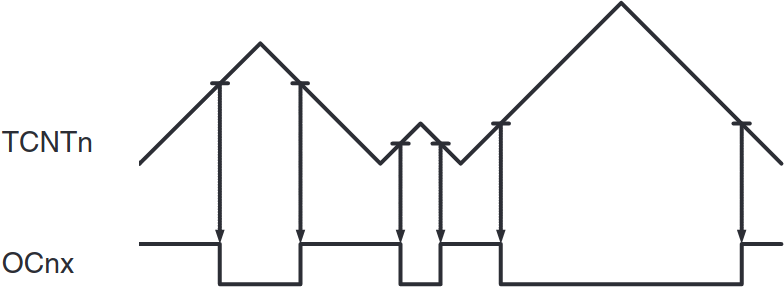
\includegraphics[width=0.9\textwidth]{felix/resources/timer_diagram.png}
    \caption{Timing diagram of the Phase and Frequency correct PWM mode}
    \label{fig:timer_diagram}
\end{figure}

\subsection{Prescaler}

The \gls{midi} protocol can encode frequencies from about 8 Hz to 13 kHz, which the timers should be able to cover. To reach this range, a prescaler can be used, which sets the counting speed of the timers to a fraction of the clock speed. Table \ref{tab:prescaler} shows all possible prescalers and their resulting frequency ranges.

Note that the maximum frequency is not actually the highest frequency possible for each prescaler. This is because the lower the number of steps, until TOP is reached, the lower the number of possible duty cycles. To ensure that for every frequency the duty cycle resolution is at least 2\%, the minimum number of steps for each period was set to 100, which effectively divides the theoretically highest possible frequency by twenty-five.

\begin{table}[h!]
    \centering
    \begin{tabular}{@{}rrrrr@{}}
        \textbf{Prescaler} & \textbf{Counting Frequency} & \textbf{Resolution} & \textbf{f\textsubscript{min}} & \textbf{f\textsubscript{max}} \\\midrule
        1 & 16 MHz & 62.5 ns & 122 Hz & 160 kHz \\
        8 & 2 MHz & 500 ns & 15.3 Hz & 20 kHz \\
        64 & 250 kHz & 4 \textmu s & 1.91 Hz & 2.5 kHz \\
        256 & 62.5 kHz & 16 \textmu s & 0.48 Hz & 625 Hz \\
        1024 & 15.625 kHz & 64 \textmu s & 0.12 Hz & 156 Hz \\
    \end{tabular}
    \caption{AAAAA}
    \label{tab:prescaler}
\end{table}

The only prescaler within the desired frequency range was the \textbf{prescaler 8}.

\subsection{Output Compare Pins}

Each Timer has three output compare units - A, B, and C - which each have their own pin, OCnA, OCnB, and OCnC, respectively. Unit B was chosen for all timers, whose pins can be seen in table \ref{tab:compare-pins}.

\begin{margintable}
\centering
\label{tab:compare-pins}
\caption{Output compare pins}
\begin{tabular}{lr}
    \textbf{MCU pin} & \textbf{Arduino pin}\\\midrule
    OC1B & 12\\
    OC3B & 2\\
    OC4B & 7\\
    OC5B & 39
\end{tabular}
\end{margintable}

\section{Using the Timers}

To use the timers in a convenient way, a timer handler has been implemented as shown in listing \ref{lst:pwmtimer}.

\begin{lstlisting}[caption=PWMTimer class, label=lst:pwmtimer]
// Constructor
PWMTimer::PWMTimer(uint16_t _ocnb_port_addr,
				   uint16_t _ocnb_pin_addr,
				   uint16_t _top_addr,
				   uint16_t _com_addr,
				   uint16_t _TCCRnA_addr,
				   uint16_t _TCCRnB_addr, 
				   uint16_t _TCNTn_addr) {
    // Save register addresses for later
    top_addr = _top_addr;
    com_addr = _com_addr;
    TCCRnB_addr = _TCCRnB_addr;
    TCNTn_addr = _TCNTn_addr;
    // Set OCnx as output
    _SFR_MEM8(_ocnb_port_addr) |= (1 << _ocnb_pin_addr);
    // Set Phase and Frequency correct PWM Mode with OCRnA as TOP
    _SFR_MEM16(_TCCRnA_addr) |= (1 << WGMn0);
    _SFR_MEM16(_TCCRnB_addr) |= (1 << WGMn3);
    // Clear OCnB on Compare Match when upcounting, set when downcounting
    _SFR_MEM16(_TCCRnA_addr) |= (1 << COMnB1);
}

void PWMTimer::start(uint16_t freq, uint8_t duty_cycle) {
    uint16_t top = 1000000 / freq;
    _SFR_MEM16(top_addr) = top;
    _SFR_MEM16(com_addr) = top * duty_cycle / 100;
    // Set prescaler to 8 to start timer
    _SFR_MEM8(TCCRnB_addr) |= (1 << CSn1);
}

void PWMTimer::stop() {
    // Wait until OCnB is low, before turning off the timer
    while(_SFR_MEM16(TCNTn_addr) < (top * duty_cycle / 100));
    // Set prescaler to 0 to stop the timer
    _SFR_MEM8(TCCRnB_addr) &= ~(1 << CSn1);
}
\end{lstlisting}

\section{Signal Combination}